\section{}

\subsection{Review of Last Lecture}
We wrote down an equation of motion for the displacement field:
\begin{equation}
    \overbrace{\rho \p_t^2 u_j}^{\text{inertia}} + \overbrace{\Gamma \p_t u_j}^{\text{drag}} = B\p_j \p_i u_i + G \nabla^2 u_j + A\e_{jk}\p_k \p_i u_i + K^0\e_{jk}\nabla^2 u_k
\end{equation}
what we keep on the LHS depend on whether we work in the overdamped/underdamped limit. What is present on the RHS depends on the terms that appear in the constitutive equation $\sigma_{ij} = K_{ijmn}u_{mn}$. $B$ is the bulk modulus, $G$ is the shear modulus, $A, K^0$ are the odd moduli - $A$ couples to the antisymmetric part of the stress tensor and gives rise to torque. $K^0$ relates to the shears, and can arise even if $\sigma_{ij} = \sigma_{ji}$.

We consider the overdamped limit where the $\rho\p_t^2 u_j$ inertia term vanishes. We also take $K^0 \gg B, A, G$ - this is a peculiar thing to do if we want to study waves, because we are overdamped and have no rigidity ($B, G \sim 0$). But we shall see such a medium can host phonons - perturbing such a system could inject enough motion to make the system go through a cycle (which could then repeat), and overcome the energy dissipated by the drag. There are some conditions that must be met for this to be observed. We start with an intuitive/heuristic argument, then proceed to write down the phase diagram/stability of such phonons more concretely.


\subsection{Phonons in damped odd solids - heuristic argument}

We consider motion of radius $R$ in displacement space $(u_x, u_y)$:

\begin{center}
    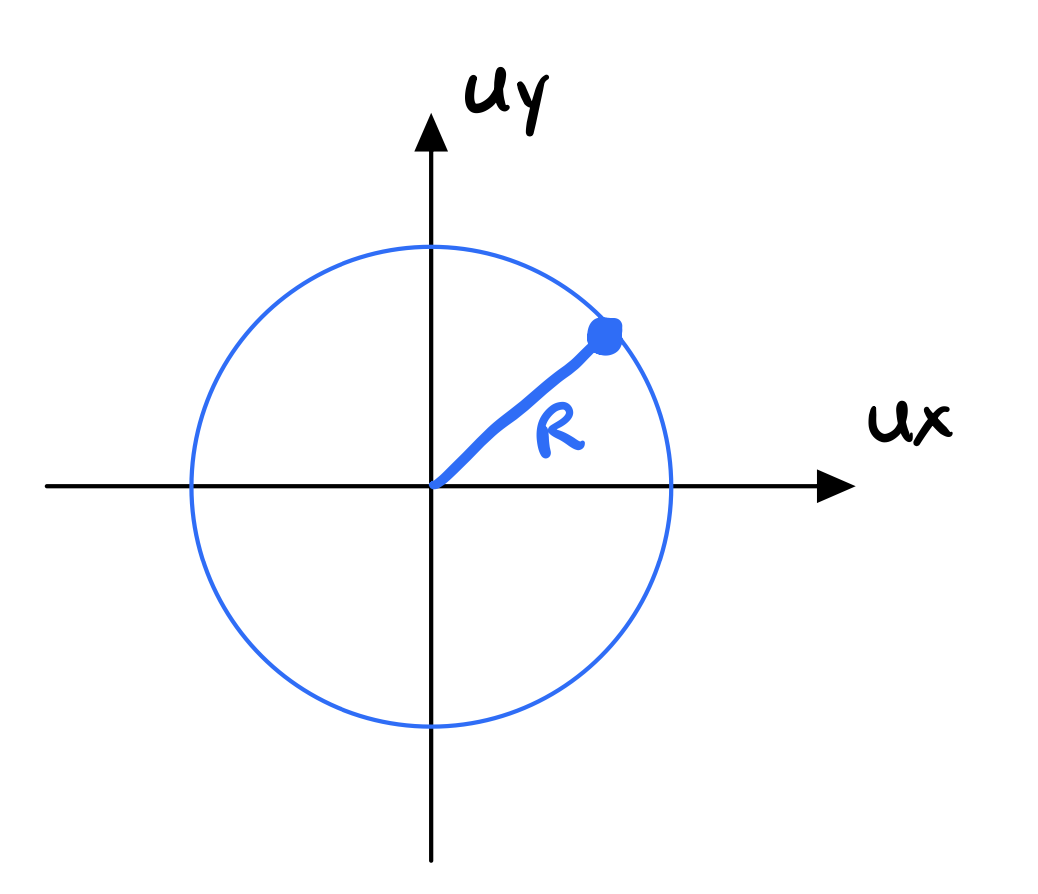
\includegraphics[scale=0.35]{Lectures/Images/lec5-uxuyspace.png}
\end{center}

Then in strain space $(S_1, S_2)$ we have a circle of radius $qR$ will be traced out over one cycle. The work done is (as we have previously calculated):
\begin{equation}
    W_{\text{odd}} = 2K^0 \cdot \text{Area} = 2K^0\pi(qR)^2
\end{equation}
Where does this energy go? We can imagine that this energy is dissipated in each cycle, so that the wave neither dies down, nor does it get amplified without bound. So, let us write down the energy being dissipated, and then balance this with the work done. The dissipated energy is:
\begin{equation}
    W_{\text{dis}} = P\Delta t = \Gamma\abs{\dot{u}}^2T = \Gamma\left(\frac{2\pi R}{T}\right)^2 T = \Gamma (2\pi R)^2 \frac{1}{T} = \Gamma R^2 2\pi \omega
\end{equation}
where $T$ is the period of the cycle. Note in the third equality that we rewrite $\dot{u}$ to be the perimeter divided by the period, and in the last equality we replace $\omega = \frac{2\pi}{T}$. Now, doing an energy balance argument, we say that the energy gained is lost by the dissipation:
\begin{equation}
    W_{\text{odd}} = W_{\text{dis}} \implies 2K^0\pi(qR)^2 = \Gamma R^2 2\pi \omega \implies \boxed{\omega = \frac{K^0}{\Gamma}q^2}
\end{equation}
Note that since the conclusion only tells us that $\omega \sim \frac{K^0}{\Gamma}q^2$ since the heuristic derivation should not necessarily give us the correct prefactor (though it does, here - a more careful derivation gives the same result). 

Note that the wave speed is given by:
\begin{equation}
    c = \frac{K^0 q}{\Gamma}
\end{equation}
so the speed of the wave scales with the wavevector/momentum $q$. Different parts of the spectrum travel at different speeds! Why no square root? We do \emph{not} have an inertial wave, where we would have two time derivatives and hence a $\omega^2$. Instead we have a dispersive wave. Note that if we take $K^0 \to 0$ (the limit of the medium becoming conservative) or take $\Gamma \to \infty$, then the wave speed goes to zero/the waves vanish.

An important note; if we have EoM $\ddot{x} = -kx$, then $k = \frac{\delta^2 U}{\delta x^2}$, we can write it as a variation of the energy. But, given that we have an odd component, $K^0_{ijmn} \neq \frac{\delta \e}{\delta u_{ij}\delta u_{mn}}$, we \emph{cannot} write it as a variation of energy. This is an example of us taking a system of solids - where traditionally everything is written as the variation of an energy - and generalizing it to a dynamical system. The dispersions we will generate as a result will have different character than what we would normally encounter in physics, either classical or quantum.

\subsection{Phonons in damped odd solids - formal argument}
Next, we want to calculate the dispersion relationship formally, and derive the phase diagram to see for what regions/phases in parameter space are phonons stable. We have equation of motion:
\begin{equation}
    \Gamma\p_t u_j = K_{ijmn}\p_i \p_m u_n
\end{equation}
we guess the ansatz:
\begin{equation}
    u_i(\v{x}) =  u_i(\v{q})e^{-i(\v{q} \cdot \v{x} + \omega t)}
\end{equation}
Leaving the algebra as an exercise, we define the parallel and transverse components:
\begin{equation}
    u_\parallel \equiv \hat{q}_i \tilde{u}_i
\end{equation}
\begin{equation}
    u_\perp \equiv \e_{ij}\hat{q}_i \tilde{u}_j
\end{equation}
then the outcome of the exercise would be:
\begin{equation}
    q_i q_m K_{ijmn}\tilde{u}_n = q^2\m{B + G & K^0 \\ -K^0 - A & G}\m{u_\parallel \\ u_\perp}
\end{equation}
If we also write the LHS in terms of $u_\parallel, u_\perp$ then:
\begin{equation}
    -i\omega \Gamma\m{u_\parallel \\ u_\perp} = -q^2\m{B + G & K^0 \\ -K^0 - A & G}\m{u_\parallel \\ u_\perp}
\end{equation}
We can then diagonalize to find the normal frequencies/modes, wherein we shall find:
\begin{equation}
    \omega = -i\left[\frac{B}{2} + G \pm \sqrt{\left(\frac{B}{2}\right)^2 - K^0A  - (K^0)^2}\right]\frac{q^2}{\Gamma}
\end{equation}
Now, the $\frac{B}{2} + G$ term corresponds to an exponential decay. It is proportional to $B, G$. There is something very subtle happening here. We perturb our solid, starting a cycle that generates energy due to $K^0, A$. The bulk and shear moduli $B, G$ do not like the cycles in strain space - from their perspective these cycles cost energy. The presence of the elastic moduli causes the damping of the waves! This is in stark contrast to oscillations that come from a potential, wherein the elastic moduli support the waves.

Going back to our expression for the frequency, the onset of active waves is whenever we have oscillatory motion of the form $e^{\pm i \text{Re}(\omega)t}$. The imaginary component can only give us decay or amplification. To get a real part, we need the square root term to be imaginary. For this, we require that the argument of the square root is negative. Thus the condition for active waves is (defining $\tilde{K}^0 = \frac{2K^0}{B}, \tilde{A} = \frac{2A}{B})$:
\begin{equation}
    \frac{B}{2}\left(1 -  \tilde{K}^0 \tilde{A} - \left(\tilde{K}^0\right)^2\right) < 0
\end{equation}
the phase transition then occurs on the hyperbola:
\begin{equation}
    \tilde{A} = \frac{1}{\tilde{K}^0} - \tilde{K}^0
\end{equation}
so we have the rough phase diagram:

\begin{center}
    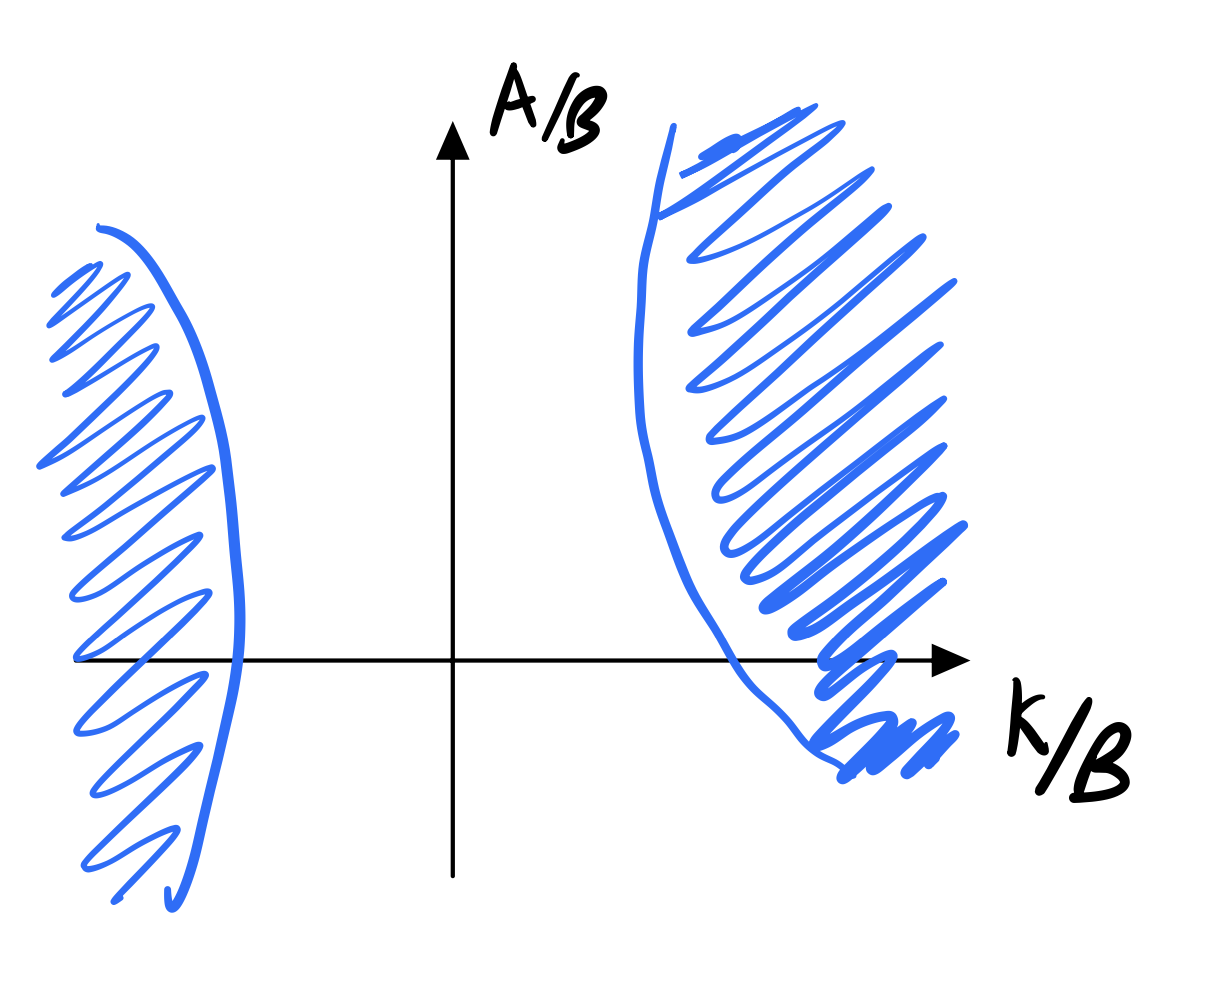
\includegraphics[scale=0.35]{Lectures/Images/lec5-phasediagram.png}
\end{center}

where in the blue regions/phases we get active waves, and in the central condition we have no propagation.

Next class we look at this phase diagram more carefully. We also look at what happens along the $ \tilde{A} = \frac{1}{\tilde{K}^0} - \tilde{K}^0$ lines and look for exceptional points. We also look at limits of large odd elastic moduli and see cases where we have amplification.